The biggest change to the current system, will be the addition of GPSs in the bikes.
This will bring the following changes:
\begin{itemize}
\item Bike stations will be completely obsolete, instead 'hot-spots' will be introduced.
\item It will be possible to track the position of bikes.
\item It will be possible to track the usage of bikes and predict future locations.
\end{itemize}

As of now, bike stations serve a limited purpose.
They are where people are supposed to place the bikes after use, thus making it possible for other people to find the bikes.
However, bikes are not necessarily returned to a station after use, somewhat disrupting the sole purpose of the bike stations.

Furthermore, by adding GPSs to the bikes, it will be possible to get an exact location of a bike, even if it is not at a bike station.
By periodically requesting the location of the bikes, their movements could be tracked.
Further, by detecting long stops (meaning ended trip), so-called hot-spots could be determined.
These hot-spots would work as informal stations, where bikes are more likely to be placed after usage.
Then it would be possible, by looking at the history of bike usage, to predict to which hot-spot a given bike is headed, when taken in to use from a certain hot-spot.

By requesting GPS locations on bikes, it will be possible to get an overview of all bikes.
This can be useful for users, who are trying to locate an available bike nearby.
It can also be used by Aalborg Kommune, to locate missing or stolen bikes.

In regards to users locating bikes, they should have a more limited view, as compared to Aalborg Kommune.
They should be restricted to viewing bikes that are available.
As of now, it is not completely certain how a bike will be confirmed available, but the main idea is to do so after a given period of time with no activity.

If a bike should leave the Aalborg area, Aalborg Kommune should be notified.
If a bike is inactive for too long, it could mean that it is broken or parked too far away for anyone to use it.
Then Aalborg Kommune could be notified, and someone can be sent to either make repairs or move it.

\begin{figure}
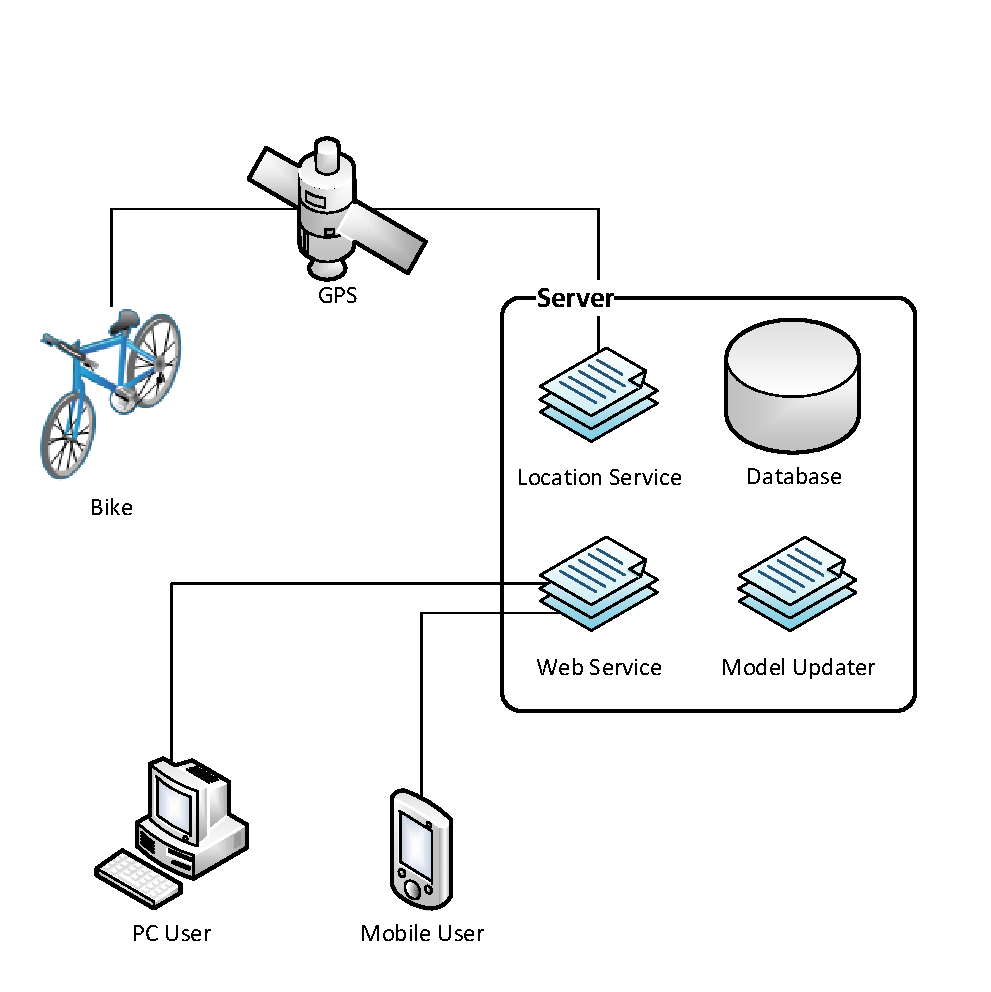
\includegraphics[width=\textwidth]{our_solution.pdf}
\caption{The overall structure of our solution}
\end{figure}
